%% tese_lncc.tex
%%
%% A última versão deste modelo está em
%%   https://github.com/equipe-customizacao-tese-lncc/tese_lncc
%%
%% Criado por:
%% Weslley da Silva Pereira
%% Lucas dos Santos Fernandez
%% Fortià Vila Verges
%%
%% Modificado por:
%% Equipe de customização - Fortià Vila Verges,
%%   Lucas dos Santos Fernandez, Weslley da Silva Pereira
%%
%% Este trabalho consiste de tese_lncc.tex,
%% abntex2lncc.sty e bibliografia.bib
%%

% ------------------------------------------------------------------------
% ------------------------------------------------------------------------
% Modelo de Trabalho Academico (tese de doutorado, dissertacao de
% mestrado e trabalhos monograficos em geral) em conformidade com
% ABNT NBR 14724:2011: Informacao e documentacao - Trabalhos academicos -
% Apresentacao
% ------------------------------------------------------------------------
% ------------------------------------------------------------------------

\documentclass[
	% -- opções da classe memoir --
	12pt,				% tamanho da fonte
	openright,			% capítulos começam em pág ímpar (insere página vazia caso preciso)
	oneside,			% para impressão em frente e verso use twoside
	a4paper,			% tamanho do papel.
	% -- opções da classe abntex2 --
	%chapter=TITLE,		% títulos de capítulos convertidos em letras maiúsculas
	%section=TITLE,		% títulos de seções convertidos em letras maiúsculas
	%subsection=TITLE,	% títulos de subseções convertidos em letras maiúsculas
	%subsubsection=TITLE,% títulos de subsubseções convertidos em letras maiúsculas
	sumario=tradicional,% sumário tradicional, com tabulação
	% -- opções do pacote babel --
	brazil,			% idioma adicional para hifenização
	french,				% idioma adicional para hifenização
	spanish,			% idioma adicional para hifenização
	english				% o último idioma é o principal do documento (mude se precisar)
	]{abntex2}

% ---
% Pacotes básicos
% ---
\usepackage{lmodern}			% Usa a fonte Latin Modern			
\usepackage[T1]{fontenc}		% Selecao de codigos de fonte.
\usepackage[utf8]{inputenc}		% Codificacao do documento (conversão automática dos acentos)
\usepackage{lastpage}			% Usado pela Ficha catalográfica
\usepackage{indentfirst}		% Indenta o primeiro parágrafo de cada seção.
\usepackage{color}				% Controle das cores
\usepackage{graphicx}			% Inclusão de gráficos
\usepackage{microtype} 			% para melhorias de justificação
\usepackage{abntex2lncc}		% Formatacao especifica do modelo do LNCC
% ---
		
% ---
% Pacotes adicionais, usados apenas no âmbito do Modelo Canônico do abnteX2
% ---
\usepackage{lipsum}				% para geração de dummy text
% ---

% ---
% Pacotes de citações
% ---
\usepackage[brazilian,hyperpageref]{backref}	 % Paginas com as citações na bibl
\usepackage[alf]{abntex2cite}	% Citações padrão ABNT
\usepackage{multirow}           % permite mesclar linhas e colunas em tabelas

% ---
% CONFIGURAÇÕES DE PACOTES
% ---

% ---
% Configurações do pacote backref
% Usado sem a opção hyperpageref de backref
\renewcommand{\backrefpagesname}{Citado na(s) página(s):~}
% Texto padrão antes do número das páginas
\renewcommand{\backref}{}
% Define os textos da citação
\renewcommand*{\backrefalt}[4]{
	\ifcase #1 %
		Nenhuma citação no texto.%
	\or
		Citado na página #2.%
	\else
		Citado #1 vezes nas páginas #2.%
	\fi}%
% ---

% ---
% CONFIGURAÇÕES DE USUÁRIO
% ---
	
% ---
% Pasta principal de imagens e logo do LNCC
\graphicspath{img}
\logoLNCC{logo/lncc}
% ---

% ---
% Tipo de trabalho (apenas uma das opções abaixo deve estar descomentada)
%\dissertacaoMestrado
\teseDoutorado
% ---

% ---
% Título
\titulo{Uncertainty Quantification Management System}
% Nome do aluno
\nomeAutor{Noel}{Moreno Lemus}
% Nome do orientador
\nomeOrientador{Fábio André}{Machado Porto}
% Coorientador(es)
% \coorientador{José Oliveira Pereira}
%\coorientador[Coorientadores:]{Coorientador 1 e Coorientador 2}
% ---

% ---
% Local
\local{Petrópolis, RJ - Brasil}
% Data
\data{Junho de 2017}
% Instituição
\instituicao{%
  Laboratório Nacional de Computação Científica
  \par
  Programa de Pós-Graduação em Modelagem Computacional}
% ---

% ---
% O preambulo deve conter o tipo do trabalho, o objetivo,
% o nome da instituição e a área de concentração
% portugues
%\preambulo{\tipoTrabalho submetida ao corpo docente do Laboratório Nacional de Computação Científica como parte dos requisitos necessários para a obtenção do grau de \grau em Ciências em Modelagem Computacional.}
%ingles
\preambulo{\tipoTrabalho submitted to the examining committee in partial fulfillment of the requirements for the degree of \grau of Sciences in Computational Modeling.}
% ---

% ---
% FICHA CATALOGRÁFICA
%
% Representa o código que sua tese/dissertação terá nos registros de  nossa biblioteca.
%
% Observação: Ao terminar de escrever sua tese/dissertação e a mesma for aprovada pela comissão de avaliação para a defesa, favor se dirigir a biblioteca.
% ---
\codebib{XXX.XXX}
\codetese{XXXX}
% ---

% ---
% Configurações de aparência do PDF final

\definecolor{blue}{RGB}{41,5,195}

% informações do PDF
\makeatletter
\hypersetup{
     	%pagebackref=true,
		pdftitle={\@title},
		pdfauthor={\@author},
    	pdfsubject={\imprimirpreambulo},
	    pdfcreator={LaTeX with abnTeX2},
		pdfkeywords={abnt}{latex}{abntex}{abntex2}{trabalho acadêmico},
		colorlinks=true,       		% false: boxed links; true: colored links
    	linkcolor=blue,          	% color of internal links
    	citecolor=blue,        		% color of links to bibliography
    	filecolor=magenta,      		% color of file links
		urlcolor=blue,
		bookmarksdepth=4
}
\makeatother
% ---

% ---
% Espaçamentos entre linhas e parágrafos
% ---

% O tamanho do parágrafo é dado por:
\setlength{\parindent}{1.3cm}

% Controle do espaçamento entre um parágrafo e outro:
\setlength{\parskip}{0.2cm}  % tente também \onelineskip

% ---
% compila o indice
% ---
\makeindex
% ---

% ----
% Início do documento
% ----

\begin{document}

% Seleciona o idioma do documento (conforme pacotes do babel)
\selectlanguage{english}
%\selectlanguage{brazil}

% Retira espaço extra obsoleto entre as frases.
\frenchspacing

% ----------------------------------------------------------
% ELEMENTOS PRÉ-TEXTUAIS
% ----------------------------------------------------------
% \pretextual

% ---
% Capa
% ---
\imprimircapa
% ---

% ---
% Folha de rosto
% (o * indica que haverá a ficha bibliográfica)
% ---
\imprimirfolhaderosto*
% ---

% ---
% Inserir a ficha bibliografica
% ---

% Isto é um exemplo de Ficha Catalográfica, ou ``Dados internacionais de
% catalogação-na-publicação''. Você pode utilizar este modelo como referência.
% Porém, provavelmente a biblioteca da sua universidade lhe fornecerá um PDF
% com a ficha catalográfica definitiva após a defesa do trabalho. Quando estiver
% com o documento, salve-o como PDF no diretório do seu projeto e substitua todo
% o conteúdo de implementação deste arquivo pelo comando abaixo:
%
% \begin{fichacatalografica}
%     \includepdf{fig_ficha_catalografica.pdf}
% \end{fichacatalografica}

\begin{fichacatalografica}
	\sffamily
	\vspace*{\fill}					% Posição vertical
	\begin{center}					% Minipage Centralizado
	\fbox{
	\begin{minipage}[c][5cm][t]{1.5cm}
	\small
	\imprimirCodeTese
	\end{minipage}
	\begin{minipage}[c][8cm][c]{13.5cm}		% Largura
	\small
	\imprimirUltimoSobrenome,{ }\imprimirNomeAutor
	%Sobrenome, Nome do autor
	
	\hspace{0.5cm} \imprimirtitulo{ }/ \imprimirautor. --
	\imprimirlocal, \imprimirdata-
	
	\hspace{0.5cm} \pageref{LastPage} p. : il. \pagColoridas ; 30 cm.\\
	
	\hspace{0.5cm} \imprimirOrientadoresRotulo~\imprimirorientador
	{ e }\imprimircoorientador\\
	
	\hspace{0.5cm}
	\parbox[t]{\textwidth}{\imprimirtipotrabalho~--~\imprimirinstituicao,
	\imprimirdata.}\\
	
	\hspace{0.5cm}
		1. Palavra-chave1.
		2. Palavra-chave2.
		2. Palavra-chave3.
		I. \imprimirUltimoSobrenomeOrientador,{ }\imprimirNomeOrientador.
		II. LNCC/MCTI.
		III. \labelTitulo

	\begin{center}
		CDD: \imprimirCodeBib	
	\end{center}		
	\end{minipage}}
	
	\end{center}
\end{fichacatalografica}
% ---

% ---
% Inserir folha de aprovação
% ---

% Isto é um exemplo de Folha de aprovação, elemento obrigatório da NBR
% 14724/2011 (seção 4.2.1.3). Você pode utilizar este modelo até a aprovação
% do trabalho. Após isso, substitua todo o conteúdo deste arquivo por uma
% imagem da página assinada pela banca com o comando abaixo:
%
% \includepdf{folhadeaprovacao_final.pdf}
%
\begin{folhadeaprovacao}

  \begin{center}
    {\ABNTEXchapterfont\large\imprimirautor}

    \vspace*{\fill}\vspace*{\fill}
    \begin{center}
      \ABNTEXchapterfont\bfseries\Large\imprimirtitulo
    \end{center}
    \vspace*{\fill}

    \hspace{.45\textwidth}
    \begin{minipage}{.5\textwidth}
        \imprimirpreambulo
    \end{minipage}%
    \vspace*{\fill}
   \end{center}

   \aprovadaPor

   \assinatura{\textbf{Prof. \imprimirorientador, D.Sc.} \\ (Presidente)}
   \assinatura{\textbf{Prof. Minch Yoda, M.Sc.}}
   \assinatura{\textbf{Prof. Kendall E. Atkinson, Ph.D.}}
   \assinatura{\textbf{Prof. Isaac Newton}}
   \assinatura{\textbf{Prof. Alan Mathison Turing, Ph.D.}}

   \begin{center}
    \vspace*{0.5cm}
    {\large\imprimirlocal}
    \par
    {\large\imprimirdata}
    \vspace*{1cm}
  \end{center}

\end{folhadeaprovacao}
% ---

% ---
% Dedicatória
% ---
\begin{dedicatoria}
   \vspace*{\fill}
   \vspace*{10cm}
   \flushright
   \noindent
   \textbf{\dedicatorianame\\}
   \textit{To my little and special family.\\} \vspace*{\fill}
\end{dedicatoria}
% ---

% ---
% Agradecimentos
% ---
\begin{agradecimentos}
O autor manifesta reconhecimentos às pessoas e instituições que colaboraram para a execução de seu trabalho.

\end{agradecimentos}
% ---

% ---
% Epígrafe
% ---
\begin{epigrafe}
    \vspace*{\fill}
	\begin{flushright}
		\textit{``Essentially, all models are wrong, but some are useful.''\\
		(George Edward Pelham)}
	\end{flushright}
\end{epigrafe}
% ---

% ---
% RESUMOS
% ---

% resumo no idioma principal
\setlength{\absparsep}{18pt} % ajusta o espaçamento dos parágrafos do resumo
\begin{resumo}
 Segundo a \citeonline[3.1-3.2]{NBR6028:2003}, o resumo deve ressaltar o
 objetivo, o método, os resultados e as conclusões do documento. A ordem e a extensão
 destes itens dependem do tipo de resumo (informativo ou indicativo) e do
 tratamento que cada item recebe no documento original. O resumo deve ser
 precedido da referência do documento, com exceção do resumo inserido no
 próprio documento. (\ldots) As palavras-chave devem figurar logo abaixo do
 resumo, antecedidas da expressão Palavras-chave:, separadas entre si por
 ponto e finalizadas também por ponto.

 \textbf{\palavrasChave}: latex. abntex. editoração de texto.
\end{resumo}

% resumo em inglês
\begin{resumo}[Abstract]
 \begin{otherlanguage*}{english}
   This is the english abstract.

   \textbf{Keywords}: latex. abntex. text editoration.
 \end{otherlanguage*}
\end{resumo}

%% resumo em português-br
%\begin{resumo}[Resumo]
% \begin{otherlanguage*}{brazil}
%    Este é um resumo em português do Brasil.
%
%   \textbf{Palavras-chave}: latex. abntex. editoração de texto.
% \end{otherlanguage*}
%\end{resumo}

%% resumo em francês
%\begin{resumo}[Résumé]
% \begin{otherlanguage*}{french}
%    Il s'agit d'un résumé en français.
%
%   \textbf{Mots-clés}: latex. abntex. publication de textes.
% \end{otherlanguage*}
%\end{resumo}

%% resumo em espanhol
%\begin{resumo}[Resumen]
% \begin{otherlanguage*}{spanish}
%   Este es el resumen en español.
%
%   \textbf{Palabras clave}: latex. abntex. publicación de textos.
% \end{otherlanguage*}
%\end{resumo}
% ---

% ---
% inserir lista de figuras
% ---
\pdfbookmark[0]{\listfigurename}{lof}
\listoffigures*
\cleardoublepage
% ---

% ---
% inserir lista de tabelas
% ---
\pdfbookmark[0]{\listtablename}{lot}
\listoftables*
\cleardoublepage
% ---

% ---
% inserir lista de abreviaturas e siglas
% ---
\begin{siglas}
  \item[ABNT] Associação Brasileira de Normas Técnicas
  \item[abnTeX] ABsurdas Normas para TeX
\end{siglas}
% ---

% ---
% inserir lista de símbolos
% ---
\begin{simbolos}
  \item[$ \Gamma $] Letra grega Gama
  \item[$ \Lambda $] Lambda
  \item[$ \zeta $] Letra grega minúscula zeta
  \item[$ \in $] Pertence
\end{simbolos}
% ---

% ---
% inserir o sumario
% ---
\pdfbookmark[0]{\contentsname}{toc}
\tableofcontents*
\cleardoublepage
% ---



% ----------------------------------------------------------
% ELEMENTOS TEXTUAIS
% ----------------------------------------------------------
\textual

% ----------------------------------------------------------
% Capítulos
% ----------------------------------------------------------
\chapter[Introduction]{Introduction}\label{cap:intro}
The rapid growth of high-performance computing and the advances in numerical techniques in the last two decades have provided an unprecedented opportunity to explore complex physical phenomena using large-scale spatio-temporal modeling and simulation.  At the same time, scientific community is leaving behind the traditional deterministic approach, which offers  point predictions with no associated uncertainty \cite{Johnstone2015};  to include Uncertainty Quantification (\textit{UQ}) as a common practice in their researches. 

Large-scale spatio-temporal simulations with quantified uncertainty enable scientists to make precise statements about the degree of confidence they have in their simulation-based predictions. These approaches find practical applicability in models for predicting the behavior of weather, hurricane forecasts \cite{Tobergte2013}, subsurface hydrology \cite{Baroni2014a}, geology \cite{Guerra2016}, nuclear reactor design, financial portfolios \cite{Chen2008}, and biological phenomena, just to name a few. They also allow to study physical phenomena that are impossible to assess experimentally, for example: simulate nuclear accidents, or the conditions that some spatial vehicle will find at landing in Mars, and so on. The success of these techniques has made them increasingly important tools for high impact predictions and decision making.

\textit{UQ}  includes different aspects that warranty the predictive fidelity of a numerical simulation, such as the uncertainty in the experimental data, which is used for defining the parameter values of a model; the propagation of uncertain  parameters through the model; and the choice of the model itself. \textit{UQ} is a complex process that covers the following main tasks: (i) uncertainty characterization \cite{Crespo2014}, also called model calibration \cite{Farrell2015a} or statistical inverse problem \cite{Estacio-Hiroms2012};  (ii) sensitivity analysis; (iii) forward problem or uncertainty propagation; and (iv) model selection.

This paper is focused on  \textit{forward propagation}, whose objective is to quantify the uncertainties in model output(s) propagated from uncertain inputs. The targets of \textit{forward propagation} analysis can be: (i) evaluate low-order moments ( i.e. mean and variance) of the outputs, (ii) evaluate the reliability of the outputs, and/or (iii) assess the complete probability distribution (\textit{PDF}) of the outputs.

When dealing with large-scale spatio-temporal models, a huge among of data is generated as a result of the simulation process. Indeed, on each spatio-temporal location $(s_{i},t_{j}) \in \mathcal{S} \times \mathcal{T}\subseteq\mathbb{R}^{3}\times\mathbb{R}$ , usually more than $10^4$ simulations are performed. Then, the size of the output dataset is in the order of $N_{s}\times N_{t}\times N_{sim}$, where: $N_{s}$ is the number of spatial locations, $N_{t}$ is the number of time steps, and $N_{sim}$ is the number of simulations.  An example of the volume of data generated by these simulations is given in the experimental section \ref{Experiments} of this paper, where the output dataset is about 2.4 TB. This turn \textit{forward propagation} in a data intensive problem.

Another important aspect, which is often not taken into account, is that the uncertainty need to be quantified in some way that can be used after, to answer questions that arise in the \textit{UQ} context. In that sense, assess the complete \textit {PDF} could be the best way to quantify uncertainty, because if you can find the \textit {PDF} that best fit the dataset with reasonably accurately, you can get all the statistical properties under one roof. At the same time, we can substitute the original data by the \textit {PDFs}, which represents a huge reduction in the volume of data to manipulate.

Contradictorily, statistical moments (e.g. mean and standard deviation) are possibly the most used ways to quantify the uncertainty, despite the fact that they doesn't have information about the manner in which the data are distributed \cite{Lampasi2006}. This is because of the difficulty to find the \textit{PDF} that best fit a dataset \cite{Karian2011},  even more, when dealing with large-scale spatio-temporal models where the \textit{PDF} needs to be derived on each spatio-temporal location, and therefore the  \textit{forward propagation} problem becomes time consuming and computationally intensive too.

However, the use of low order moments alone prevents us from making accurate analysis with respect to the uncertainty. They are not enough neither for the characterization nor for the quantification of the uncertainty, and questions such as:
\begin{itemize}
\item What is the uncertainty in the spatio-temporal region $\mathcal{S}_{i} \times \mathcal{T}_{j}$ associated to the \textit{QoI} 
$q_{k}$  and a computational model $\mathcal{M}_{m}$?
\item How to compare different spatio-temporal regions $\mathcal{S}_{i} \times \mathcal{T}_{j}$ with respect to the uncertainty? 
\item What is the less uncertain model from the set of models $\mathcal{M}={\mathcal{M}_{1},\mathcal{M}_{2},
....\mathcal{M}_{m}}$, to predict the value of a QoI $q_{k}$, over a spatio-temporal region $\mathcal{S}_{i} \times \mathcal{T}_{j}$?
\end{itemize}
can be poorly answered. So, we emphasize that only the characterization of the uncertainty by using the \textit{PDF} allows aware decisions.

A first effort to try to estimate the \textit{PDFs} on large-scale spatio-temporal simulations was done by \cite{Liu2018} {Ji et. al.} in \textbf{\textit{Parallel Computation of PDFs on Big Spatial Data Using Spark}}. They propose a new solution to efficiently compute the \textit{PDFs} in parallel using Spark, through three methods: data grouping, machine learning prediction and sampling. The main drawback of the proposed approach is that you should try many different distributions, to find the PDF that best fits the dataset on each specific spatio-temporal location. Another drawback is that, as we mentioned above, the uncertainty needs to be quantified in the way that facilitates its further use; and the heterogeneity of the functions used in the approach doesn't facilitate it. 

To face these challenges, in this paper we propose a general framework to quantify the uncertainty in large-scale spatio-temporal models. It uses a data-driven approach and combines the generalized lambda distribution (\textit{GLD}), clusters algorithms and information entropy, for helping researchers to answer the above questions and many others that arise in \textit{UQ} context. Our proposal provides a generally applicable and easy-to-use tool that supports the representation and analysis of uncertainty, as was suggested in the "\textit{Workshop on Quantification, Communication, and Interpretation of Uncertainty in Simulation and Data Science}" \cite{Tobergte2013}. 

In order to illustrate the use of the proposed framework, a case study is discussed. The main results obtained are: (i) the \textit{GLD} good fits for more than the 80 \% of the dataset, (ii) the use of the \textit{GLD} allows to include clustering algorithms to group the spatio-temporal locations with similar uncertainty, (iii) the centroids  of the clusters can be used as a faithful representation of the rest of the spatio-temporal locations, which significantly reduces the data corresponding to the simulation outputs, (iv) with the use of these centroids we can characterize the uncertainty in any spatio-temporal region as a mixture of \textit{GLDs}.

The rest of the paper is organized as follows: Section \ref{UQBackground} gives the theoretical foundations of \textit{UQ} and highlights some interesting aspects included in our proposal. Section \ref{materials_methods} describes the principal characteristics of the \textit{GLD} that make it suitable for this proposal. Section \ref{Approach} presents the proposed approach, the workflow we implement and some considerations of the implementation. Section \ref{Experiments} presents a use case and discusses the results. This use case allows us to explain our approach in the context of a real problem, which facilitates its understanding. Section \ref{RelatedWorks} covers the related works and finally, section \ref{Conclusions} concludes the paper and proposes some future works.

\section{Research Objectives}

\begin{tcolorbox}
The main objective of this thesis is the proposal of a new method to quantify the uncertainty in large-scale spatio-temporal models based on the Generalized Lambda Distribution (GLD).
\end{tcolorbox}

To achieve that goal the following research questions need to be answered:

\textbf{RQ1.} how to group the output of the UQ process based on the similarity of the uncertainty?

\textbf{RQ2.} what is the uncertainty in some spatio-temporal locations not previously analysed?

\textbf{RQ3.} what is the uncertainty of an specific spatio-temporal region?

\textbf{RQ4.} how to compare two regions as a function of its uncertainty?

\textbf{RQ5.} what is the less uncertain model from a set of models?

\textbf{RQ1} and \textbf{RQ2} are answered in chapter \ref{cap:gld_clustering}, while \textbf{RQ3}, \textbf{RQ4} and \textbf{RQ5} are answered in chapter \ref{cap:our_approach}. In chapter \ref{cap:use_cases} all the questions are answered again for all the use cases.

\section{Highlights of the Dissertation}

\section{Organization of the Dissertation}

The structure of the remainder of this thesis is outlined for reference.

\textbf{Chapter 2} background of UQ.

\textbf{Chapter 3} Ji paper.

\textbf{Chapter 4} GLD.

\textbf{Chapter 5} GLD clustering and kriging.

\textbf{Chapter 6} Workflow.

\textbf{Chapter 7} Use cases.

\textbf{Chapter 8} Conclusions and future works.

%% abtex2-modelo-include-comandos.tex, v-1.9.6 laurocesar
%% Copyright 2012-2016 by abnTeX2 group at http://www.abntex.net.br/
%%
%% This work may be distributed and/or modified under the
%% conditions of the LaTeX Project Public License, either version 1.3
%% of this license or (at your option) any later version.
%% The latest version of this license is in
%%   http://www.latex-project.org/lppl.txt
%% and version 1.3 or later is part of all distributions of LaTeX
%% version 2005/12/01 or later.
%%
%% This work has the LPPL maintenance status `maintained'.
%%
%% The Current Maintainer of this work is the abnTeX2 team, led
%% by Lauro César Araujo. Further $\infty$ormation are available on
%% http://www.abntex.net.br/
%%
%% This work consists of the files abntex2-modelo-include-comandos.tex
%% and abntex2-modelo-img-marca.pdf
%%

% ---
% Este capítulo, utilizado por diferentes exemplos do abnTeX2, ilustra o uso de
% comandos do abnTeX2 e de LaTeX.
% ---

\chapter{Uncertainty Quantification Background}\label{cap:backgroud}


\begin{flushright}
	\textit{``UQ cannot tell you that your model is 'right' or 'true', \\
	but only that, if you accept the validity of the model (to some \\
	quantified degree), then you must logically accept the validity\\
	of certain conclusions (to some quantified degree)''\\
	\cite{Sullivan2015}}
\end{flushright}

Uncertainty quantification (UQ) is a topic of great importance and hence widespread interest in computational analyses that are used to support important societal decisions on issues related to climate change [15-19], reactor safety [20-26], radioactive waste disposal [27-34], nuclear weapon safety [35-38], economic policy [39-43], environmental degradation [44- 47], and many additional areas of concern and challenge. Indeed, it is difficult to envision how adequately informed decisions can be made on such issues without an appropriate assessment of the uncertainties present in the supporting analyses.

In this chapter, we summarize some definitions in UQ context that are important to understand the rest of the document. Also, different ways of representation of the uncertainty are discussed, with a brief justification of those we are going to use in the thesis. A general workflow of the UQ process is presented where we contextualize our contributions. A detailed discussion about forward propagation is presented. And finally, we summarize the chapter.

All results of interest can be derived from the PDF \cite{Cox2012}.

In particular it is not always convenient to retain the M = 106, say, (vector) values produced by MC and use them subsequently \cite{Cox2012}.

\section{Definitions}
\subsection{Errors vs Uncertainties}

The mismatch between the true physical phenomena and the prediction obtained by modeling and simulation (M\&S) process can arise from the mathematical representation of a real problem, a physical problem (are the values of the parameters a good representation of the reality?), a computational problem (translation of a mathematical formulation into a numerical algorithm and a computational code) \cite{Thibaut2015}. Uncertainty and error can be considered as the broad categories  that  are  normally  associated to this mismatch. Until recently terms  uncertainty  and error  have  commonly  been  used  interchangeably.  It is believed, however, that failure to distinguish between these terms is detrimental to the quantification of credibility in M\&S. According to \cite{Oberkampf1998} we can classify errors and uncertainties as follow: 

\begin{itemize}
\item[•] \textbf{errors:} recognizable deficiencies of the model or the algorithms employed. Errors are associated to: physical approximations to simplify the modeling of a physical process, translation of the mathematical to computational model, numerical approximations (truncation or roundoff), etc. When the errors are knowns there are reasonable means of estimating the magnitude of the error introduced. 
\item[•] \textbf{uncertainties:} potential deficiency that is due to lack of knowledge. The different sources of uncertainty can be:
\begin{itemize}
\item[-] \textbf{parameter uncertainty}, which comes from the model parameters that are inputs to the computer model (mathematical model) but whose exact values are unknown to experimentalists and cannot be controlled in physical experiments, or whose values cannot be exactly inferred by statistical methods. Examples are the local free-fall acceleration in a falling object experiment, various material properties in a finite element analysis for engineering, and multiplier uncertainty in the context of macroeconomic policy optimization \cite{Kennedy2001}.
\item[-] \textbf{model inadequacy}, no model is perfect. Even if there is no parameter uncertainty, so that we know the true values of all the inputs required to make a particular prediction of the process being modeled, the predicted value will not equal the true value of the process. The discrepancy is model inadequacy. Since the real process may itself exhibit random variability, we define model inadequacy to be the difference between the true mean value of the real world process and the code output at the true values of the inputs.
\item[-] \textbf{parametric variability}, which comes from the variability of input variables of the model. For example, the dimensions of a work piece in a process of manufacture may not be exactly as designed and instructed, which would cause variability in its performance. 
\item[-] \textbf{structural uncertainty}, aka model inadequacy, model bias, or model discrepancy, which comes from the lack of knowledge of the underlying true physics. It depends on how accurately a mathematical model describes the true system for a real-life situation, considering the fact that models are almost always only approximations to reality. One example is when modeling the process of a falling object using the free-fall model; the model itself is inaccurate since there always exists air friction. In this case, even if there is no unknown parameter in the model, a discrepancy is still expected between the model and true physics. 
\item[-] \textbf{algorithmic uncertainty}, aka numerical uncertainty, which comes from numerical errors and numerical approximations per implementation of the computer model. Most models are too complicated to solve exactly. For example, the finite element method or finite difference method may be used to approximate the solution of a partial differential equation, which, however, introduces numerical errors. Other examples are numerical integration and infinite sum truncation that are necessary approximations in numerical implementation. 
\item[-] \textbf{experimental uncertainty}, aka observation error, which comes from the variability of experimental measurements. The experimental uncertainty is inevitable and can be noticed by repeating a measurement for many times using exactly the same settings for all inputs/variables. 
\item[-] \textbf{interpolation uncertainty}, which comes from a lack of available data collected from computer model simulations and/or experimental measurements. For other input settings that don't have simulation data or experimental measurements, one must interpolate or extrapolate in order to predict the corresponding responses.
\end{itemize}
\end{itemize}

A more elegant definition of what uncertainty is, is enunciated in \cite{Helton2009} as:

\begin{defn}
Uncertainty is a best estimate of the range of a particular metric which may derive from one or two broad sources. Uncertainties that reflect a lack of knowledge about the appropriate value to use for a quantity that is assumed to have (missing modifier: a fixed?) value in the context of a particular analysis are termed \textbf{\textit{epistemic}}. Uncertainties that arise from an inherent randomness in the behavior of the system under study are termed \textbf{\textit{aleatoric}}.
\end{defn}

\subsection{Aleatoric vs Epistemic Uncertainty}

It is sometimes assumed that uncertainty can be classified into those two categories, \textbf{\textit{aleatoric}} and \textbf{\textit{epistemic}}, although the validity of this categorization is open to debate \cite{Kiureghian2009}. 

\textbf{Aleatoric uncertainty} arises from an inherent randomness in the properties or behavior of the system under study. For example, the weather conditions at the time of a reactor accident are inherently random with respect to our ability to predict the future. Other examples include the variability in the properties of a population of weapon components and the variability in the possible future environmental conditions that a weapon component could be exposed to. Alternative designations for \textbf{aleatory uncertainty} include variability, stochastic, irreducible and type A. \cite{Helton2009}

\textbf{Epistemic uncertainty} derives from a lack of knowledge about the appropriate value to use for a quantity that is assumed to have a fixed value in the context of a particular analysis. For example, the pressure at which a given reactor containment would fail for a specified set of pressurization conditions is fixed but not amenable to being unambiguously defined. Other examples include minimum voltage required for the operation of a system and the maximum temperature that a system can withstand before failing. Alternative designations for \textbf{epistemic uncertainty} include state of knowledge, subjective, reducible and type B. \cite{Helton2009}

While \textbf{epistemic uncertainty} can be reduced through experiments, improvement of the numerical methods and so on, \textbf{aleatory uncertainty} can not be reduced. 


\subsection{Uncertainty Quantification}

UQ is not a mature field like linear algebra or single-variable complex analysis, with stately textbooks containing well-polished presentations of classical theorems bearing August names like Cauchy, Gauss and Hamilton. Both because of its youth as a field and its very close engagement with applications, UQ is much more about problems, methods and ‘good enough for the job’. There are some very elegant approaches within UQ, but as yet no single, general, overarching theory of UQ. \cite{Sullivan2015}

UQ neither have a unique and globally accepted definition. In the reviewed literature we find some definitions that, from our point of view, are those that batter describe what UQ is.  

In the Wikipedia we find the following definition: 

\begin{defn}
Uncertainty Quantification is the science of quantitative characterization and reduction of uncertainties in applications. It tries to determine how likely certain outcomes are if some aspects of the system are not exactly known.
\end{defn}

This definition is very general and may be ignore some important aspects, by as a first approach is a good one. 

In October of 2009 the U.S. Department of Energy organize a comission to study the impact of Extreme Scale computing in its National Security. One of the aspects analysed by the comision was UQ. In the report \textit{"Scientific Grand Challenges in National Security: The Role of Computing at the Extreme Scale"} \cite{DEnergy2009}, the authors define UQ as:

\begin{defn}
Uncertainty Quantification (UQ) studies all sources of error and uncertainty, including the following:  
systematic and stochastic measurement error; ignorance; limitations of theoretical models; limitations of 
numerical representations of those models; limitations of the accuracy and reliability of computations, 
approximations, and algorithms; and human error. A more precise definition is UQ is the end-to-end 
study of the reliability of scientific inferences. \cite{DEnergy2009}
\end{defn}

A more recent definition was introduced by Higdon et al. \cite{Higdon2017} in the \textit{"Handbook of Uncertainty Quantification"}:

\begin{defn}
Uncertainty Quantification is the rational process by which proximity between predictions and observations is characterized. It can be thought of as the task of determining appropriate uncertainties associated with model-based predictions. More broadly, it is a field that combines concepts from applied mathematics, engineering, computational science, and statistics, producing methodology, tools, and research to connect computational models to the actual physical systems they simulate. In this broader interpretation, UQ is relevant to a wide span of investigations. These range from seeking detailed quantitative predictions for a well-understood and accurately modeled engineering systems to exploratory investigations focused on understanding trade-offs in a new or even hypothetical physical system. \cite{Higdon2017}
\end{defn}

Just to remark, in this definition the sentence: \textbf{a field that combines concepts from applied mathematics, engineering, computational science, and statistics, producing methodology, tools, and research to connect computational models to the actual physical systems they simulate}, illustrate the multidisciplinary nature of UQ and the main objectives of this research field.


\section{Uncertainty Representation}

An immediate challenge in the development of an appropriate treatment of uncertainty is the selection of a mathematical structure to be used in its representation \cite{Helton2010}. Traditionally, probability theory has provided this structure [48-55]. However, in the last several decades, additional mathematical structures for the representation of uncertainty such as evidence theory [56-63], possibility theory [64- 70], fuzzy set theory [71-75], and interval analysis [76-81] have been introduced.
This introduction has been accompanied by a lively discussion of the strengths and weaknesses of the various mathematical structures for the representation of uncertainty [82-90]. For perspective, several comparative discussions of these different approaches to the representation of uncertainty are available [72; 91-98].

%\cite{Helton2010a}

This section briefly summarizes some of this approaches, and discuss in more details probability theory as this is the main one used in the rest of the thesis.

\subsection{Interval Analysis}

\subsection{Variance}

\subsection{Information Entropy}
\label{InformationEntropy}
The concept of information entropy was first defined by Shannon (1948) in a study performed to identify the amount of information required to transmit English text. The underlying idea was that, given the probabilities of letters occurring in the English alphabet, it is possible to derive a measure describing the missing information to determine the full text of a partially transmitted message, where information is understood as the information required to identify the message, not the information of the message itself. Based on several theoretical considerations, Shannon derived the following equation to classify a measure of the missing information, often referred to as information entropy:

\begin{equation}
H=-\sum_{i}^N p_{i}\log p_{i}
\end{equation}

The information entropy \textit{H} is defined as the sum of the product of the probability \textit{p} for each possible outcome \textit{i} of \textit{N}, total possible outcomes, with its logarithm. The minimum value is 0, because $\log 1=0$. 

\subsubsection{Information entropy in a spatio-temporal context}
\label{InformationEntropySpatioTemporal}
For each spatio-temporal region, the information entropy can be described as: 

\begin{equation}\label{eq: spatio-temporal Entropy}
H(s,t)=-\sum_{m=1}^M p_{m}(s,t)\log p_{m}(s,t)
\end{equation}
where $s$ denotes the location of the subregion, $M$ represents the number of possible (exclusive) members the subregion may contain, and $t$ is the physical time.

\subsubsection{Information entropy as a meause of uncertainty}\label{subsub:informationentropytomeasuretheuncertainty}
Based on \ref{InformationEntropy} and \ref{InformationEntropySpatioTemporal}, if the possible outcomes of the model and the probability of each outcome on each $(s,t)$, are known, then the information entropy could be used as a qualitative measure of the uncertainty of the model output. For example, in a spatio-temporal region $(s,t)$ where the outcome is always the same, the information entropy is 0, because the outcome is known. On the other hand, in the worse case where all the outcomes have the same probability in $(s,t)$, the entropy is maximum and the uncertainty too.

%The main limitations of this method, is that the possible outcomes of the model are  usually not known. To tackle this problem, in section \ref{Clusterizing the GLD based in its lambda values} we present a novel algorithm that uses a clusterization method over the $\lambda$ values of the \textit{GLD}, to group the model output in possible outcomes. Then, with those outcomes we can apply Information Entropy to estimate the uncertainty on different contexts.

\subsection{Probability Theory}
Probability theory is based on the specification of a triple $(\Omega,\mathcal{F},P)$, where $\Omega$ is the set of all possible outcomes, $\mathcal{F}$  is a suitably restricted collection of subsets of $\Omega$, and $P$ defines the probability of the elements of $\Omega$.

The probability measure $P$ is a function returning an event's probability, with the properties that $0 \leq P \leq 1$ and $P(\Omega)=1$

One way to characterize the probability is through the probability density function (\textit{PDF}). It is a mathematical function that, stated in simple terms, can be thought of as providing the probabilities of occurrence of different possible outcomes in an experiment. 

\textbf{Probability density function}: for a continuous random variable $X$, we can define the probability that $X$ is in $[a,b]$ as:
\begin{equation}
P(a<=X<=b)=\int_a^b f(x)dx
\end{equation}

where $f(x)$ is a probability density function, which satisfies two properties:
\begin{equation*}
\begin{aligned}
& f(x)>=0 \\ 
& \int_{-\infty}^{+\infty}f(x) dx =1
\end{aligned}
\end{equation*}
a, b are real numbers.
The \textit{PDF} defines the probability that $X<=a$ as
$P(X<=a)=\int_{-\infty}^a f(x) dx$

\section{Some Typical UQ Problems}
Many typical UQ problems can be illustrated in the context of a system $F$, that maps input $X$ in some space $\mathcal{X}$ to outputs $Y = \mathcal{M}(X)$ in some space $\mathcal{Y}$, through a mathematical/computational model $\mathcal{M}$. Some common UQ objectives include: \textit{forward propagation or push-forward problem}, Section \ref{seq:forward}; \textit{reliability or certification problem}, Section \ref{seq:reliability}; \textit{prediction problem}, Section \ref{seq:prediction}; \textit{inverse problem}, Section \ref{seq:inverse}; \textit{sensitivity analysis}, Section \ref{seq:sensitivity}; and \textit{model reduction or model calibration problem}, Section \ref{seq:calibration}.

\begin{figure}[H]
    \centering
    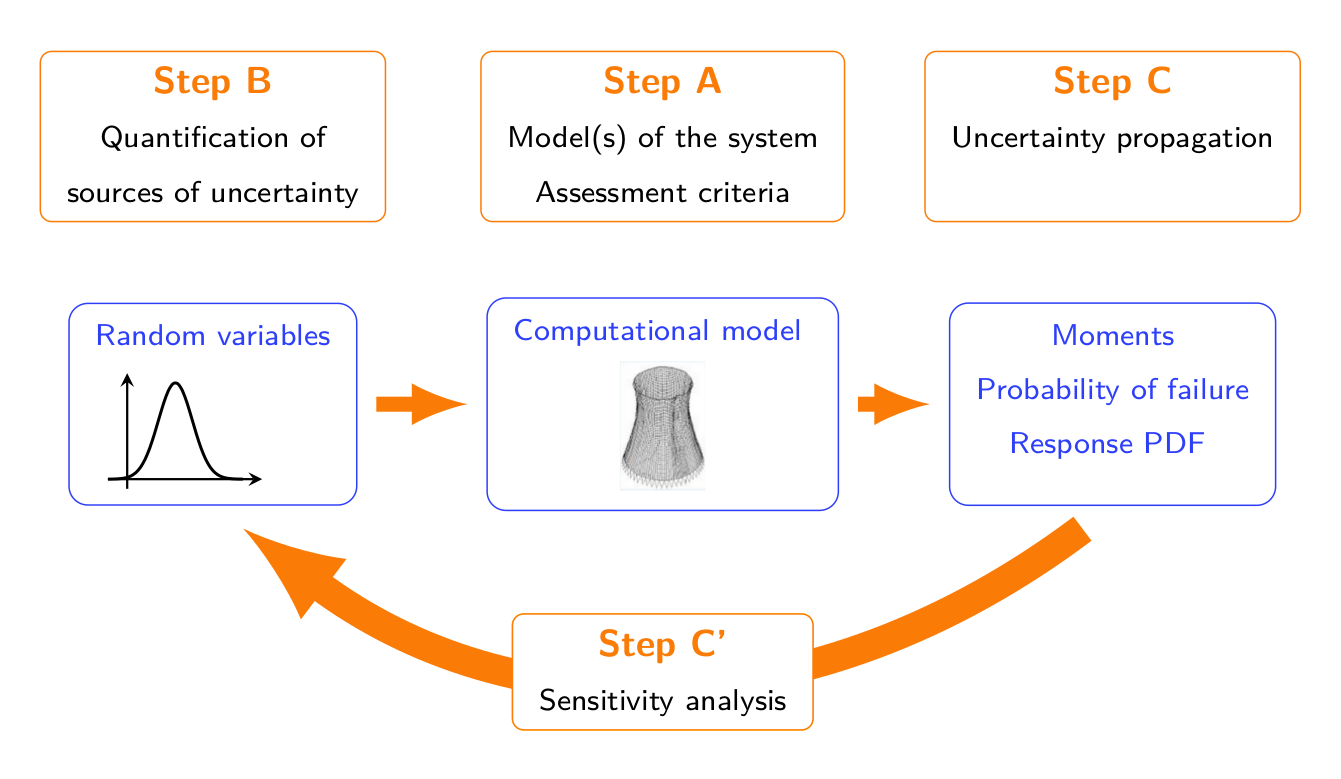
\includegraphics[width=0.8\textwidth]{img/background/UQ_steps.png}
    \caption{Uncertainty Quantification workflow. Taken from \href{http://www.uqlab.com/}{UQLab}.}
    \label{fig:uqlab_workflow}
\end{figure}

\subsection{Forward propagation or push-forward problem}\label{seq:forward}
Given the equation $\bm{Y}=\mathcal{M}(\bm{X})$ where: 
\begin{itemize}
\item $\bm{X} \in \mathcal{X} $ is a vector of  input parameters of the model,
\item $\mathcal{M}$ is a computational model, and
\item $\bm{Y} \in \mathcal{Y}$ is a vector that represents  quantities of interest (\textit{QoI}).
\end{itemize}
Suppose that the uncertainty about the inputs of $\mathcal{M}$ can be summarized in a probability distribution $P$ on $\mathcal{X}$. Then in a \textit{forward propagation}, the objective is to quantify the uncertainty of $\bm{Y}$, induced by $\bm{X}$ through $\mathcal{M}$.

The main objective of this thesis is a new method to quantify the uncertainty of the output of large-scale spatio-temporal models, that is a \textit{forward propagation problem}. In Section \ref{seq:methods_uq_propagation} some methods for \textit{forward propagation} are exposed; while in Section \ref{seq:uq_large_scale} we discuse about \textit{forward propagation} in large-scale spatio-temporal models.  

\subsection{Reliability or certification problem}\label{seq:reliability}
Suppose that some set $\mathcal{Y}_{fail}\subseteq \mathcal{Y}$ is identified as a 'failure set'. Then in a reliability analysis we are interesting in, given appropriate information about the input $X$ and a process $F$, determine the failure probability 
\begin{equation}
\mathcal{P}[\mathcal{M}(X)\in \mathcal{Y}_{fail}]
\end{equation}
Furthermore, how large will the deviation from acceptable performance be, and what are the consequences? \cite{Sullivan2015}

\subsection{Prediction problem}\label{seq:prediction}
Similar to the reliability problem, given a maximum acceptable probability error $\epsilon > 0$, find a set $\mathcal{Y}_{\epsilon}\subseteq \mathcal{Y}$ such that
\begin{equation}
\mathcal{P}[\mathcal{M}(X)\in \mathcal{Y}_{\epsilon}]\geq 1-\epsilon
\end{equation}

in other works, the prediction $\mathcal{M}(X)\in \mathcal{Y}_{\epsilon}$ is wrong with probability at most $\epsilon$.

\subsection{Inverse problem or parameter estimation}\label{seq:inverse}
Given some experimental measurements of the output $Y$ of the system and some computer simulation results from its mathematical model $\mathcal{M}$, inverse uncertainty quantification estimates the discrepancy between the experiment and the mathematical model (which is called \textit{bias correction}), and estimates the values of unknown parameters in the model if there are any (which is called \textit{parameter calibration}) \cite{GharibShirangi2014}. Generally this is a much more difficult problem than forward uncertainty propagation; however it is of great importance since it is typically implemented in a model updating process.

\subsection{Sensitivity Analysis}\label{seq:sensitivity}
Sensitivity analysis refers to the determination of the contributions of individual uncertain analysis inputs to the uncertainty in analysis results. The goal in sensitivity analysis is to apportion the uncertainty in $Y$ to the uncertainty in inputs $X$, \cite{Sankararaman2012}. 

\subsection{Model reduction or model calibration problem}\label{seq:calibration}
Construct another model $\mathcal{M}_{h}$ such that $\mathcal{M}_{h} \approx \mathcal{M}$ in an appropriate sense. 

\subsection{Model selection}
If, for the system $F$ we have a set of models $\mathcal{M} = \lbrace \mathcal{M}_{1}, \mathcal{M}_{2},...,\mathcal{M}_{n} \rbrace$, then a model selection problem consist in the selection of the most plausible model $\mathcal{M}_{i}$ that best fit the experimental data.

Sometimes a UQ problem consists of several of these problems coupled together, for example, one might have to solve an \textbf{\textit{inverse problem}} to produce or improve some model parameters, and then use those parameters to propagate some other uncertainties \textbf{\textit{forwards}}, and hence produce a \textbf{\textit{prediction}} that can be used for decision support in some \textbf{\textit{certification problem}} \cite{Sullivan2015}.

In this thesis we focus in \textbf{\textit{forward propagation problem}} although in chapter \ref{cap:use_cases} we introduce some queries that help to solve \textbf{\textit{reliability or certification}} and \textbf{\textit{prediction problem}}.

\section{Methods for Uncertainty Propagation}\label{seq:methods_uq_propagation}

\subsection{Sampling Methods}

\subsubsection{Monte Carlo}
To date, the MC simulation is the most powerful method for the uncertainty evaluation, \cite{Rajan2016a}.

Monte Carlo simulations (MCS) provide the most robust and straightforward way to
solve PDEs with random coefficients. In the case of (22.2), for instance, they consist
of (i) generating multiple realizations of the input parameters a and b, (ii) solving
deterministic PDEs for each realization, and (iii) evaluating ensemble statistics or
PDFs of these solutions. MCS do not impose limitations on statistical properties of
input parameters, entail no modifications of existing deterministic solvers, and are
ideal for parallel computing \cite{Higdon2017}.

\section{UQ in Large-scale Spatio-temporal models}\label{seq:uq_large_scale}
The emerging field of data science is largely lacking in generalizable methods for quantifying the uncertainty in the output of analysis systems. As a result, a major new research initiative needs to be initiated in this area. Since data science programs are just getting established in universities, this effort needs to be accompanied by relevant curriculum development \cite{Tobergte2013}

%The question of how to represent and communicate uncertainties is a topic of research both from a practical and theoretical point of view. A fair bit of theoretical research is aimed at the mathematical calculus of uncertainty. This includes extensions and alternatives to standard probabilistic reasoning, such as Dempster-Schafer theory and imprecise probabilities. When uncertainties are needed for investigations requiring computational models, additional considerations arise. For example, if the simulation output is a daily surface-temperature field over the globe for the next 200 years, representing uncertainty and dependencies is complex. Should ensembles be used to represent plausible outcomes? How should these ensembles of simulation output be stored? How can high-consequence/low-probability outcomes be discovered in this massive output? Here some research investigations attempt to leverage theory that exploits high dimensionality to bound probabilities and system behavior. Finally, even when uncertainties are well captured, how best to communicate such uncertainties to the public or to decision-makers is also a topic of ongoing research. 
%\cite{DEnergy2009}

\section{Software and Tools for UQ}
Currently, advances in uncertainty propagation and assessment have been paralleled by a growing number of software tools for uncertainty analysis, but none has gained recognition for a universal applicability, including case studies with spatial models and spatial model inputs. \cite{Sawicka2016}

These include both free software, like OpenTURNS (Andrianov et al., 2007), DACOTA (Adams et al., 2009) and DUE (Brown and Heuvelink, 2007), commercial, like COSSAN (Schuëller and Pradlwarter, 2006), or free, but written for a licenced software, e.g. SAFE (Pianosi et al., 2015) or UQLab (Marelli and Sudret, 2014) toolboxes for MATLAB. A broad review of existing software packages is available in Bastin et al. (2013). To the best of our knowledge, however, none of the existent software is specifically designed to be extended by the environmental science community. The use of powerful but complex languages like C++ (e.g. Dakota), Python (e.g. OpenTURNS) or Java (e.g. DUE) often discourages relevant portions of the non-highly-IT trained scientific community from the adoption of otherwise powerful tools.
spup-R package \cite{Sawicka2016}. De aqui saque lo de arriba tambien, aunque lo de arriba lo puedo buscar en sus respectivos papers y hablar un poco de cada uno de ellos.

\section{Summary}

\section{Concepts}
high-dimensional parameter spaces \cite{DEnergy2009}
computationally demanding forward models 
nonlinearity and/or complexity in the forward model

\section{Ideas a usar}
HPC and computational modeling play a dominant role in shaping the methodological developments and research in uncertainty qualification. Depending on the complexity of the uncertainty qualification investigation, anywhere from $10^{2}$ to $10^{8}$ runs of the computational model may be required. Thus, uncertainty qualification investigations may require extreme-computing environments (e.g., exascale) to obtain results in a useful time frame, even if a single run of the computational model does not require such resources. \cite{DEnergy2009}

Advances in computing over the past few decades—both in availability and power—have led to an explosion in computational models available for simulating a wide variety of complex physical (and social) systems. These complex models—which may involve millions of lines of code, and require extreme-computing resources—have led to numerous scientific discoveries and advances. This is because these models allow simulation of physical processes in environments and conditions that are difficult or even impossible to access experimentally. However, scientists’ abilities to quantify uncertainties in these model-based predictions lag well behind their abilities to produce these computational models. This is largely because such simulation-based scientific investigations present a set of challenges that is not present in traditional investigations.

\cite{DEnergy2009}

Until recently, the original approach of describing model parameters using single values has been retained, and consequently the majority of mathematical models in use today provide point predictions, with no associated uncertainty. \cite{Johnstone2015}

a 'typical' UQ problem involves one or more mathematical models for a process of interest, subject to some uncertainty about the correct form of, or parameter values for, those models. \cite{Sullivan2015}

Often, though not always, these uncertainties are treated probabilistically. \cite{Sullivan2015}

but how will you actually go about evaluating that expected value when it is an integral over a million-dimensional parameter space?
Practical problems from engineering and the sciences can easily have models with millions or billions of inputs
(degrees of freedom). \cite{Sullivan2015}

the language of probability theory is a powerful tool in describing uncertainty \cite{Sullivan2015}

“UQ studies all sources of error and uncertainty, including the following: systematic and stochastic measurement error; ignorance; limitations of theoretical models; limitations of numerical representations of those models; limitations of the accuracy and reliability of computations, approximations, and algorithms; and human error. A more precise definition is UQ is the end-to-end study of the reliability of scientific inferences.” \cite{DEnergy2009} (U.S. Department of Energy, 2009, p. 135)



In \cite{Sullivan2015} the authors remark that is important to appreciate both the underlying mathematics and the practicalities of implementation. In his work they focus in the presentation of the former and keep the latter in mind. In our work we do the opposite, we focus in the implementation keeping the math formalism in mind.

Probability theorists usually denote the sample space of a probability space by $\Omega$; PDE theorists often use the same letter to denote a domain in $\Re^{n}$ on which a partial differential equation is to be solved. In UQ, where the worlds of probability and PDE theory often collide, the possibility of confusion is clear. Therefore, this book will tend to use $\Theta$ for a probability space and \textbf{X} for a more general measurable space, which may happen to be the spatial domain for some PDE.

\chapter[Uncertainty Quantification Process]{Uncertainty Quantification Process}\label{cap_uq_process}

\section[Measures of Information and Uncertainty]{Measures of Information and Uncertainty}

\subsection{Variance, Information and Entropy}

\textbf{Variance.} 

\textbf{Information and Entropy.}

\subsection{Information Gain, Distances and Divergences}

\section{Sensitivity Analysis}
Sensitivity analysis is the systematic study of how model inputs—parameters, initial and boundary conditions—affect key model outputs. Depending on the application, one might use local derivatives or global descriptors such as Sobol’s functional decomposition or variance decomposition. Also, the needs of the application may range from simple ranking of the importance of inputs to a response surface model that predicts the output given the input settings. Such sensitivity studies are complicated by a number of factors, including the dimensionality of the input space, the complexity of the computational model, limited forward model runs due to the computational demands of the model, the availability of adjoint solvers or derivative information, stochastic simulation output, and high-dimensional output. Challenges in sensitivity analysis include dealing with these factors while addressing the needs of the application. \cite{DEnergy2009}

\begin{equation}
E=mc^2
\end{equation}
\chapter{UQMS Data Model}\label{cap_data_model}

\section{Introduction}

\section{SaViMe}

\section{UQMS Data Model}

\section{UQMS Operations}

\chapter{Implementation of the UQMS in Tensorflow}\label{cap_tensorflow}

\section{Why Tensorflow}

\subsection{Variables in Tensorflow}

\subsection{Operations in Tensorflow}

%\chapter{Case Study: Seismic Example}\label{cap_seismic}

\chapter[Applicability]{Applicability}\label{Applicability}

In the present chapter we are going to test the UQMS in three different scenarios, spatial only domain, section \ref{Wave Propagation} , spatio-temporal domain, section \ref{spatio_temporal}, and finally a multidisciplinary system, section \ref{NASA}. 

\section{Case Study:  Wave Propagation Problem}\label{Wave Propagation}

The first one is a geophysical tests for wave propagation problems

As a first case study we use the “HPC4E Seismic Test Suite”, a collection of four 3D models and sixteen associated tests that can be downloaded freely at the project's website (https://hpc4e.eu/downloads/datasets-and-software ). The models include simple cases that can be used in the development stage of any geophysical imaging practitioner (developer, tester ...) as well as extremely large cases that can only be solved in a reasonable time using ExaFLOPS supercomputers. The models are generated to the required size by means of a Matlab/Octave script and hence can be used by users of any OS or computing platform. The tests can be used to benchmark and compare the capabilities of different and innovative seismic modelling approaches, hence simplifying the task of assessing the algorithmic and computational advantages that they pose. %\cite{deLaPuente2015}

In our case, we are going to use the “HPC4E Seismic Test Suite” as a case study of the porposed UQMS. As we mention in the introduction of this chapter this model is a spatial only domain problem, because we are going to consider a multidimentional array as an Input and a multidimentional array as an output, but of them time independet.

\subsection{Mathematical Formulation}

\subsection{Model and Dataset Description}
The models have been designed as a set of 16 layers with constant physical properties. The top layer delineates the topography and the other 15 different layer interface surfaces or horizons. In the following, an interface horizon is associated with properties that apply to the layer that exists between itself and the immediately next layer horizon. The model covers an area of 10 x 10 x 5 km, with maximum topography at about 500 m and maximum depth at about 4500 m. The layer horizons have been sampled very finely with 1.6667 m spacing so that a highly accurate representation can be honored at high frequencies. For simulation schemes based on unstructured grids, the layer horizons can be used easily to constrain model blocks. For simulation schemes based upon Cartesian grids, a simple script is provided that can generate 3D grids for any desired spatial sampling. Table \ref{layers_constants} shows the properties of each of the layers included in the models. %\cite{deLaPuente2015}

\begin{table}[]
\centering
\caption{Layer constant properties and their depth range. “Star” layers are only used in the flat case, in substitution of their non-star equivalents}
\label{layers_constants}
\begin{tabular}{|l|l|l|l|l|l|}
\hline
\multicolumn{1}{|c|}{\textbf{\begin{tabular}[c]{@{}c@{}}Layer\\ Id\end{tabular}}} & \multicolumn{1}{c|}{\textbf{\begin{tabular}[c]{@{}c@{}}Vp\\ (m/s)\end{tabular}}} & \multicolumn{1}{c|}{\textbf{\begin{tabular}[c]{@{}c@{}}Vs\\ (m/s)\end{tabular}}} & \multicolumn{1}{c|}{\textbf{\begin{tabular}[c]{@{}c@{}}Density\\ (Kg/m3)\end{tabular}}} & \multicolumn{1}{c|}{\textbf{\begin{tabular}[c]{@{}c@{}}Max. depth\\ (m)\end{tabular}}} & \multicolumn{1}{c|}{\textbf{\begin{tabular}[c]{@{}c@{}}Min. depth\\ (m)\end{tabular}}} \\ \hline
1 & 1618.92 & 500.00 & 1966.38 & -135.55 & -476.35 \\ \hline
2 & 1684.08 & 765.49 & 1985.88 & 41.50 &  -394.90 \\ \hline
3 &  &  &  &  &  \\ \hline
4 &  &  &  &  &  \\ \hline
5 &  &  &  &  &  \\ \hline
6 &  &  &  &  &  \\ \hline
7 &  &  &  &  &  \\ \hline
8 &  &  &  &  &  \\ \hline
9 &  &  &  &  &  \\ \hline
10 &  &  &  &  &  \\ \hline
11 &  &  &  &  &  \\ \hline
12 &  &  &  &  &  \\ \hline
13 &  &  &  &  &  \\ \hline
14 &  &  &  &  &  \\ \hline
15 &  &  &  &  &  \\ \hline
16 &  &  &  &  &  \\ \hline
2* &  &  &  &  &  \\ \hline
3* &  &  &  &  &  \\ \hline
\end{tabular}
\end{table}

\subsection{Adding uncertainty into the model}

The “HPC4E Seismic Test Suite” does not provide uncertainty sources, because all the input parameters of the model have fixed values. Then, to the purpose of our work we need to add some uncertainties into the inputs. Let's suppose the variable ${V_{p}}$ is uncertain. As this variable have 16 different values, one for each layer, we can consider it as a random vector, equation \ref{random_vector_vp}. We associate to each of the $V_{{p}_{i}}$ a Normal distribution with ${\mu}_{i}$ equal to the value reported in Table \ref{layers_constants} and $\sigma=2$.
\begin{equation}\label{random_vector_vp}
V_{p}=<V_{{p}_{i}},\mathcal{N}({\mu}_{i},{\sigma}_{i})>
\end{equation}

\section{Case Study: Austin, queso library}\label{spatio_temporal}

\section{Case Study: Multidisciplinary System (NASA)}\label{NASA}

\section{Case Study: Spatio-temporal Nicholson-Bailey model}
Este esta en el software uqlab, en la carpeta Doc Manuals

\chapter[Validation]{Validation}\label{Validation}


% ---

% ----------------------------------------------------------
% Finaliza a parte no bookmark do PDF
% para que se inicie o bookmark na raiz
% e adiciona espaço de parte no Sumário
% ----------------------------------------------------------
\phantompart

% ---
% Conclusão
% ---
\chapter[Conclusions and Future Works]{Conclusions and Future Works}\label{cap:conclusions}
Large-scale spatio-temporal simulations produce a huge amount of data that need to be interpreted in order to assess the simulation quality in different regions of space-time. Querying these data poses a great challenge due to their volume and different data distributions. In order to solve this problem, 
in this paper we propose SUQ$^2$, a general approach to answer uncertainty quantification queries. 

The approach uses \textit{GLD} that enables the representation of a spatio-temporal simulation output using a single functional formalism. By modeling each spatio-temporal point by a GLD instance, we can synthesize the region in a number of clusters, represented by their centroid GLD function. From this basis, queries can be answered by combining the centroids in a spatio-time region into GLD-mixture functions. Moreover, by using information entropy techniques, a value can be assigned that represents the uncertainty in a region. The proposed approach is implemented in a workflow that can be extended to solve new UQ queries.

We ran extensive experiments using a seismic use case. The results showed that GLD representation of the data is valid on $85 \%$ of the dataset. Other extensions of the GLD formalism, such as EGLD \cite{Karian2011}, can be evaluated to improve the GLD dataset coverage. Moreover, we showed that the computed centroid function is a good representation of the function instances in its cluster. Additionally, we use the Kolmogorov-Smirnov test to evaluate the quality of the GLD mixture. The p-value, larger than 0.05, assures that the results of the mixture is a good representation of the raw data in the region. Finally, the adoption of the Information Entropy technique was validated by showing the correspondence of the computed values with the uncertainty in the spatio-temporal regions. 

To the best of our knowledge, this is the first work to use GLD as the basis for answering UQ queries in spatio-temporal regions and to compile a series of techniques to produce a query answering workflow.

\section{Revisiting the Research Questions}

\section{Significance and Limitations}

\section{Open Problems and Future Work}
Some of the future directions we are interested in pursuing were mentioned above. For example, in Section \ref{useCaseClustering} we mention that for the purpose of this paper we select \textit{k-means} as the clustering algorithm to be used. This arbitrary selection needs to be studied, and some algorithms implemented to provide an automatic way to cluster the \textit{GLDs}, based on the shapes described in Section \ref{gldShape}.

In Section \ref{useCaseQualityofFit}, there is a region where the \textit{GLD} does not fit well the dataset. If we want to provide a general purpose computational approach for \textit{forward propagation} we need to further investigate this issue.

The use of Information Entropy to quantify the uncertainty is very powerful. However, when applied on clusters of PDFs, such as the GLD, it observes the information variation as a function of the PDF definition, in the case of GLD this is given by its for $\lambda$ parameters. In this context, a complete region modeled by a single GLD function would have a very low information entropy value. This, however would not express the uncertainty modeled by the GLD function, which could be very high. The outcome of the information entropy evaluation must be interpreted by the user. 

\section{Final Considerations}

\subsection*{Acknowledgments}
This work has been funded by CNPq, CAPES, FAPERJ, Inria (SciDISC project) and the European Commission (HPC4E H2020 project) and performed (for E. Pacitti and P. Valduriez) in the context of the Computational Biology Institute (www.ibc-montpellier.fr) and for (F. Porto, H. Lustosa and N. Lemus) in the context of the DEXL Laboratory (dexl.lncc.br)  at LNCC.

% ---

% ----------------------------------------------------------
% ELEMENTOS PÓS-TEXTUAIS
% ----------------------------------------------------------
\postextual
% ----------------------------------------------------------

% ----------------------------------------------------------
% Referências bibliográficas
% ----------------------------------------------------------
\bibliography{MyCollection}

% ----------------------------------------------------------
% Glossário
% ----------------------------------------------------------
%
% Consulte o manual da classe abntex2 para orientações sobre o glossário.
%
%\glossary

% ----------------------------------------------------------
% Apêndices
% ----------------------------------------------------------

% ---
% Inicia os apêndices
% ---
\begin{apendicesenv}

% Imprime uma página indicando o início dos apêndices
\partapendices

% Inclusão dos arquivos referentes aos apêndices
% ----------------------------------------------------------
\chapter{Título do apêndice A}\label{apendiceA}

\lipsum[50]

\section{Título da seção}

Aqui temos uma seção dentro do Apêndice.

\begin{figure}
    \begin{center}
        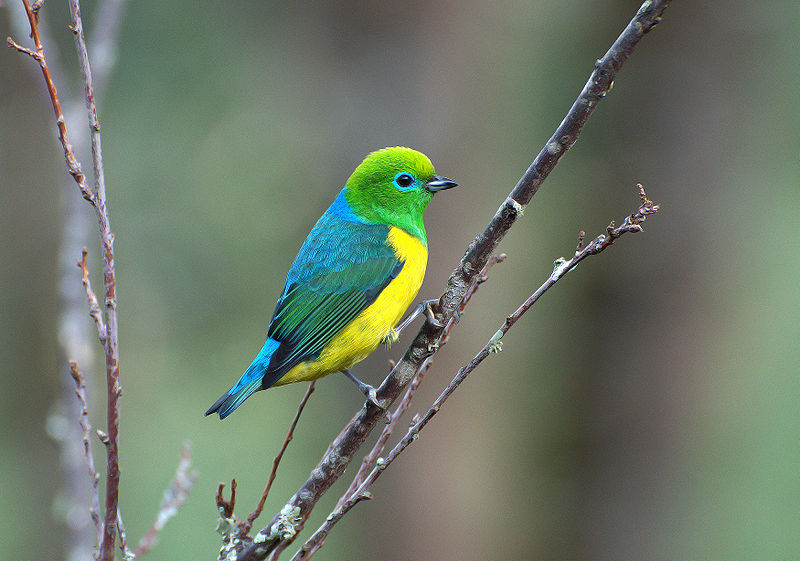
\includegraphics[width=12cm]{img/abntex2-modelo-livro-bandeirinha}
        \caption{Legenda para a figura.}
        \label{rotulo1}
    \end{center}
\end{figure}
\chapter{Título do apêndice B}\label{apendiceB}

\lipsum[55-57]

\chapter{Título do apêndice C}\label{apendiceC}

%\lipsum[9] 

% ----------------------------------------------------------

\end{apendicesenv}
% ---

% ----------------------------------------------------------
% Anexos
% ----------------------------------------------------------

% ---
% Inicia os anexos
% ---
\begin{anexosenv}

% Imprime uma página indicando o início dos anexos
\partanexos

% Inclusão dos arquivos referentes aos anexos
% ----------------------------------------------------------
\chapter{Título do anexo A}\label{anexoA}

\lipsum[23-24]

\section{Título da seção}

Aqui temos uma seção dentro do Anexo.

\lipsum[25]

\chapter{Título do anexo B}\label{anexoB}

%\lipsum[76-77]
\chapter{Título do anexo C}\label{anexoC}

\lipsum[55-57]
% ----------------------------------------------------------

\end{anexosenv}

%---------------------------------------------------------------------
% INDICE REMISSIVO
%---------------------------------------------------------------------
\phantompart
\printindex
%---------------------------------------------------------------------

\end{document}
